\chapter{Machine architecture for software designers}
\label{chap:arch}
As software designers, we may work with different mental models of the hardware
that run our programs. Particularly performance-conscious designers may be
concerned with the access speeds of CPU registers vs CPU cache. C programmers
may think of main memory and cache as a single, contiguous address-space that
they can manipulate freely. Java programmers may ignore even
the existence of the memory hierarchy altogether, and simply think about objects
and their relationships.

The purpose of this chapter is to help multicore-software designers understand the
workings of the memory hierarchy. To that end, I describe the memory hierarchy
in a manner that is abstract enough to be useful (and understandable) for the
non-hardware oriented software designer, but detailed enough to explain the
performance characteristics of e.g. false sharing.

\section{Model of the computer}
We will work with a simplified model of a computer, consisting of the following
components:

\begin{itemize}
	\item CPU cores, each with their own registers. A core executes a single
		thread at a time, or more if it uses hyper-threading.
	\item Individual CPUs, each of which may contain multiple individual cores.
	\item Per-CPU cache hierarchies, with multiple layers of cache,
		some of which are shared between multiple cores.
	\item Main memory (colloquially RAM), shared between all CPUs.
\end{itemize}

The next page shows an image of the hardware topology of a machine with two Xeon E5 CPUs,
each with 12 physical cores. The image is generaited with the Open MPI hwloc
tool.

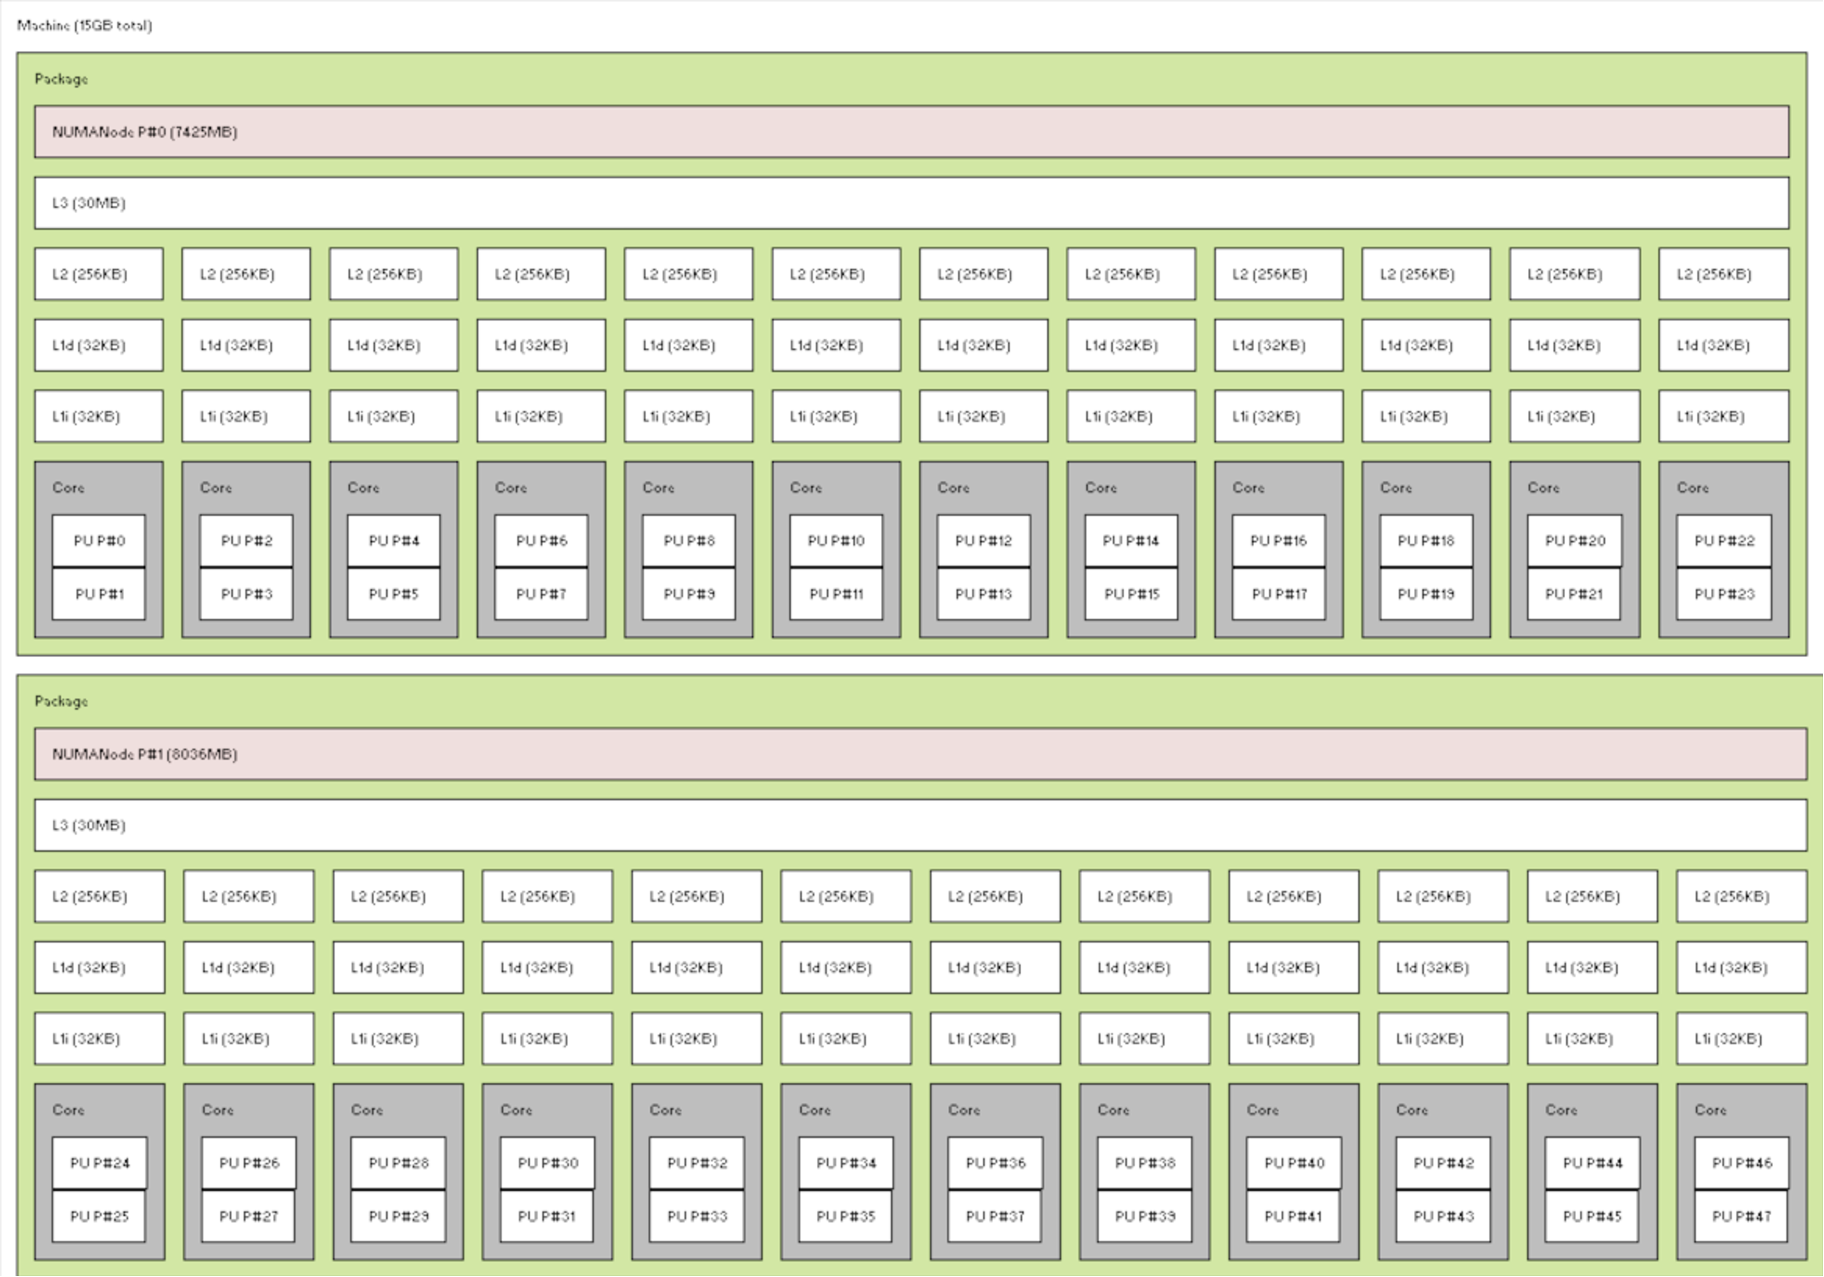
\includepdf[angle=90]{img/lstopo.pdf}

The image shows that main memory is shared between the two CPUs, each CPU has
its own L3 cache that is shared among its cores, and each physical core has its
own L2, L1d and L1i caches, shared between its virtual cores. Cache layer 1
is divided into separate caches for data (L1d) and CPU instructions (L1i).

This model excludes many aspects of real computers. Such as: The buses that
transfer data between hardware components, address-translation hardware such as
translation lookaside buffers, hard drives, and network interfaces. Each of
these may or may not have their own interesting multicore-performance
characteristics, that we shall simply ignore.

In this model, main memory is the slowest resource we work with. As we shall see
in section \ref{chap:experiments}, reading from main memory takes on the
order of 35-140 nanoseconds, whereas reading from L1 cache can be done in 1-4
nanoseconds. It follows directly from this fact that the cache-friendliness of a
program can significantly affect performance: If a program performs a billion
reads, this is the difference between a second and a few minutes.

So why not built larger caches? As commented earlier, larger caches generally
mean longer access times. Going to extremes, \citeauthor{mckenney} \cite{mckenney} notes that in order
to access storage within the time of a single 5GHz CPU-clock cycle, the storage
can be no more than 3 centimeters away from the CPU core, or we would have to
transfer the data faster than the speed of light. Furthermore; we do not (yet)
use light to transfer information between the components of a computer. We use
low-voltage electricity, which is (according to \cite{mckenney}) about 3-30
times slower.

\section{Main memory}
The main memory functions as a kind of backbone of the memory hierarchy. It is
large (often in the tens of gibibytes), and when working with high-level
languages, we tend to think about the entire memory
hierarchy in terms of how the main memory works: A contiguous storage space,
divided into fixed chunks of equal size, each of which can be
accessed individually using fixed-width addresses. This "fixed-width" is
generally what is meant when we say an architecture is "x-bit": A 64-bit
architecture uses memory addresses that are 64-bit long, and has 64-bit long
words.

\section{CPU caches}
\label{sec:caches}
Regardless of how the software designer thinks of memory, the CPU cache is not
generally a part of their interface: cache access happens transparently as we
access the main memory. It is not however transparent with
respect to performance, and cache-sympathetic software design can yield
significant performance gains. A famous example of this is found in the 2012
\texttt{GoingNative} keynote by \citeauthor{stroustrup} \cite{stroustrup}, in
which he explains that insertion into linked lists is much slower than
insertion into arrays/vectors, because of the unpredictable memory access
pattern exhibited by traversing a linked list. In this section we take a look
at the performance characteristics of CPU caches, and see that cache-friendly
design in multicore programming is radically different from cache-friendly
design in single-core programming.

A word of caution:
Since the cache is mostly invisible to software designers, hardware designers
have a lot of freedom when designing them. This makes it difficult to model and
reason about cache-behaviour across platforms. This section gives an overview
of cache hardware that applies to most modern, general-purpose hardware,
including x86 and x86-64 implementations. For a more comprehensive outline of
modern memory-hardware, chapters 2, 3, and 6 of
\cite{whatprogrammersshouldknow} should be of help. However, as is usually the
case with hardware performance, the best way to determine how a program
performs with respect to the cache is to run benchmarks on the platform
it will run on.

\subsection{What is cached and how} The cache works by storing copies
of data from main memory. That way, the cache provides faster access to
memory contents we expect to access in the future.

We could think of caches as general key-value stores, associating memory
addresses with cached values. Such a cache could let us cache values for any
set of memory locations we would like, subject only to the space constraints of
the cache. This type of cache (called \textit{fully associative}) scales
poorly as it would have to store the memory addresses in addition to the cached
values. Furthermore, any read or write operation must search the cache for an
entry with the relevant memory address. While this may sound simple enough to
software designers, cache behaviours are implemented as electronic circuitry.
For these reasons, large caches -- such as the multi-kibibyte L1 caches closest
to the CPU cores -- are not fully associative. Instead, set-associative caches
are used \cite{whatprogrammersshouldknow} \cite{mckenny-barriers}.

A set-associative cache is like is a hardware hash table with probing and
fixed-sized buckets -- or "sets". Each memory address hashes to a specific set,
and each set can contain a fixed number of entries, called "ways". The hash
function simply takes a fixed number of the least significant bits of the
address. This eliminates the need for storing the full memory address of each
cache entry: Part of the address is implied by the set used. The need to search
the full cache is similarly eliminated: The hardware now only needs to search
within a single set.

The storage in each way in a set is called a cache line. The cache line
size can be thought of as a unit size of cache operations. The cache line size
is important, because it is effectively the unit size for memory operations that
do not explicitly bypass the cache! Most, if not all, of
Intel's x86-64 architectures use 64-byte cache lines\cite{inteloptimize}.

The downside of set-associative caches is, that unlike fully associative
caches, they cannot cache an arbitrary set of memory entries: In a 2-way
set-associative cache, only two entries whose addresses hash to the same set can
be stored at a time. If a third entry hashes to the same set, one of the two
first will be evicted from the cache, regardless of how much free space is in
the other sets. Indeed it is possible for a program to use only memory
addresses that hash to the same set, effectively only utilizing a small portion
of the cache. Since the hash function uses the least significant bits, this can
generally be avoided by keeping data close together in memory.

According to \citeauthor{whatprogrammersshouldknow}, typical
CPUs in 2007 used associativity levels of up to 24 ways for L2 and larger
caches, and 8 ways for L1 \cite{whatprogrammersshouldknow}. Intel's
optimization reference-manual \cite{inteloptimize} indicates that CPUs using their
Skylake microarchitecture (from 2015) use 8 ways in L1, 4 ways in L2, and up to
16 ways in L3, so the 2007 figures appear to be current.

Several things can cause data to be stored in cache. In general, reads by
a CPU core from main memory are stored in cache, under the
assumption that having accessed it once, the data will likely be accessed again
soon after. Similarly, the cache works as a buffer for writes to main memory:
When a CPU writes a value to a memory address it first copies the full
cache line into its own cache; then the relevant part of the cache line is
overwritten in cache. The cache line is written back to memory (or to a
cache higher up in the hierarchy) at a later time. Caches that buffer writes
like this are known as write-back caches, as opposed to write-through caches
where writes are immediately propagated into main memory.

The contents of main memory may also be cached by clever prefetch mechanisms that
anticipate future accesses. For example, iterating over the elements of an array
creates a memory access-pattern (also know as a "stride") that is easily
predictable. It may help to think of such access patterns as a function $f(n) =
\ldots$, where $n$ is the number of accesses we have already made, and $f(n)$ is
the next address we want to access. The stride of reading every third element
from an array can then be described by the linear function $f(n) = 3n$ (ignoring
the complications of array-element size, the array base-pointer, and virtual
memory).
The first access is to address $f(0) = 0$, the second to $f(1) = 3$, etc.
Individual caches have associated prefetch-hardware that essentially performs
regression-analysis of actual memory accesses in order to guess the constants of
the stride function and perform reads before they are requested. Modern
commodity hardware can generally predict strides that are linear functions.

Some hardware platforms (e.g. x64 and x86-64) also provide instructions for
prefetching; letting software designers prefetch manually if the hardware
prefetch mechanisms are unsatisfactory\cite{whatprogrammersshouldknow}.
Similarly, there are so called "non-temporal" instructions available to read and
write to main memory without the values being cached.

\subsection{Data sharing and cache coherence}
The fact that writes are buffered in the caches is our first hint that
multicore programming is non-trivial. As different CPU cores store copies
of data from main memory in their own caches (and in registers as well), it is
possible for different cores to have different ideas of what the value stored at
a certain memory address is.

\begin{figure}[ht]
	\fbox{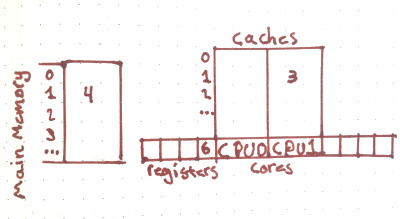
\includegraphics[width=1.0\textwidth]{img/incoherence.jpg}}
	\caption{Two CPUs with incoherent views of what is stored at memory
	location 1}
	\label{fig:incoherence}
\end{figure}

Figure \ref{fig:incoherence} shows 2 CPU cores, their registers, caches, and
shared main memory. The CPUs have reached a state where there are 3 different
values for the same memory location. None of which can be said to be more
"correct" than the others.
The state depicted in figure \ref{fig:incoherence} can be reached e.g. by the
following sequence of actions:

\begin{enumerate}
	\item Main memory has the value 4 stored at location 1.
	\item CPU1 reads location 1 from main memory, and decrements it by 1.
	\item CPU0 calculates a new value (6) in a register, and is about to
		write it to location 1.
	\item CPU1 writes the result (3) back to location 1, causing it to be
		stored in cache, but not yet in main memory.
\end{enumerate}

It is up to the software designer or compiler to avoid incoherence in CPU
registers. The remainder of this chapter is concerned with the how hardware
helps us avoid them in cache.

Multicore architectures solve such incoherences with "cache coherence
protocols". The purpose of a cache coherence protocol is to ensure that different
caches agree -- to some extent -- what the contents of a specific cache line
are. We consider the MESI protocol \cite{mesi,mckenny-barriers}, which
guarantees that at most one CPU core modifies its copy of a cache line at a
time.

Different architectures use different coherence protocols
of varying complexity.
MESI lays the foundation for the MESIF and MOESI protocols designed for Intel
and AMD respectively.

The unit of the coherence protocol is called a "coherence block". On machines
with hardware coherence, like x86 and x86-64, coherence blocks
are cache lines. On DSM and NUMA machines, they may be pages
instead\cite{falsedef}.
In this report, I use the terms cache line and coherence block interchangeably.

The MESI protocol works by attaching one of four states to each cache line
entry in each cache:

\begin{description}
\item[Modified] means the cache line is exclusive to this cache, and has been
modified by the CPU since it was cached. The cache line is invalid in the caches of all other cores.
\item[Exclusive] means the same as modified, except the cache line has not been modified since it was cached.
\item[Shared] means other caches have a copy of this cache line too.
\item[Invalid] means the cache line is not in cache. Either because it has not
been cached, or because it has been evicted, or invalidated by request of another CPU.
\end{description}

 The MESI protocol takes its name from these states.

Rather than restating the full protocol here, we will describe the most
pertinent behaviours that result from read and write operations. This is
illustrative of the protocol, and sufficient for our purposes.

The default behaviour, with little overhead or benefit from the coherence
protocol, is as follows: When a CPU core writes to cache, it must first ensure that
the cache line is in the S or M state. If it is not, the CPU core must send an
invalidation message to all other CPUs. The other CPU cores must then, upon
receiving the invalidation message, set the cache
line state to I and respond with an acknowledge message. If one of the other
CPUs has the cache line in the M state, it will send the value of the cache line
along with the acknowledge message. Other CPU cores may be able to "snoop" the
returned value into their caches as well, if they are connected to an
interconnect between the requesting and responding cores. Read operations work
the same way, but the other CPU cores set the cache line state to S instead of I.

To avoid stalling, when a core performs a write it does not actually wait
for the acknowledge messages. Instead it records the write to its per-core store
buffer, and continues execution. Later, when the cache line arrives in its
cache, the buffered value is written into the cache. Similarly, when receiving
an invalidation message, the core does not immediately invalidate the cache
line. It sends back the acknowledge message -- along with the cached value if the
cache line is set as M -- and then queues the actual invalidation in a per-core
invalidation queue. The
CPU core will however process the invalidation before sending any other messages
regarding that cache line\cite{mckenny-barriers}.

The guarantees provided by the coherence protocol by default are very weak.
To reap the benefits of the coherence protocol, we must endure its full
overhead. Software designers achieve this by using memory barrier
instructions. Different sets of memory barrier instructions are provided by
different operating systems and architectures. What matters to us is that some
of them are used to force CPU cores to flush the store buffers and to process the
invalidation queues, causing momentary coherence between the cores that execute
them. Essentially, memory barriers cause the CPU cores to stall while they perform
coherence operations.

It bears repeating that cache operations are always performed in accordance with
the coherence protocol, regardless of whether or not we use memory barriers.
This means the overhead of sending invalidation and acknowledge messages is
always present. The memory barriers affect the use of store buffers and
invalidation queues, thus improving coherence and increasing the coherence
overhead.

\subsection{False sharing of cache lines}
If two CPU cores write to the same memory location, the coherence block or cache
line containing that location is passed from one cache to the other. This is the
wanted outcome, and ensures coherence between the caches. If two CPU cores write
to \textit{different} memory locations inside the same cache line, the exact
same thing happens, but with no benefit. The coherence protocol dictates the
cache invalidations in order to achieve cache coherence, but there is no
incoherence, as the CPU cores do not share any data, just the cache line. We use
the term "false sharing of cache lines" to describe two or more CPU cores
accessing disjoint sets of data located within the same cache line. The
unnecessary cache invalidations caused by false sharing are called "false
invalidations". We use the term "false sharing overhead" to refer to the full
overhead of the coherence protocol caused by false sharing of cache lines,
including sending and processing the false invalidations.

Consider the two threads in code snippet \ref{code:falsesharing} running in
parallel on two cores. The threads never operate on the same memory location, but
if the two array elements are stored in the same cache line the cores will keep
sending false invalidation messages to each other. Without memory barriers this
causes unnecessary coherence messages to be sent back and forth, but much of the
overhead will be hidden by the store buffers and invalidation queues. With
memory barriers, the CPU cores will be forced to stall while they wait for each
other to invalidate the cache line and send the acknowledge message back.

\begin{code}
\begin{Verbatim}[frame=single]
  final int[] arr = ...;
  ...
  //Thread 0
  for(;;) {
	  arr[0]++;
  }
  ...
  //Thread 1
  for(;;) {
	  arr[1]++;
  }
  ...
\end{Verbatim}
	\caption{Pseudo code with two threads accessing different sets of data,
	that may be located in the same cache line.}
	\label{code:falsesharing}
\end{code}

The table in figure \ref{table:invalidationsequence} shows one possible sequence
of cache operations when executing the threads. The sequence in the table
assumes that the increment operations are surrounded by memory barriers, the two
array elements are in the same cache line, and that CPU0 executes thread 0 and
that CPU1 executes thread1.

\begin{figure}[hbtp]
	\centering
	\begin{tabular}{|r|c|c||c|c|}
	\hline
	& & & \multicolumn{2}{c|}{State} \\
		\cline{4-5}
	Sequence \# & CPU \# & Operation & 0 & 1\\
	\hline
	\hline
	0 & & & I & I\\
	\hline
	1 & 0 & Read & E & I\\
	\hline
	2 & 0 & Write & M & I\\
	\hline
	3 & 1 & Read & I & E\\
	\hline
	4 & 0 & Read & S & S\\
	\hline
	5 & 0 & Write & M & I\\
	\hline
	6 & 1 & Read & I & E\\
	\hline
	7 & 1 & Write & I & M\\
		\multicolumn{5}{c}{\vdots}
\end{tabular}
	\caption{Possible sequence of cache operations when executing the code
	in snippet \ref{code:falsesharing}. The values in the state column
	indicates the MESI state of the shared cache line in the caches of CPU0
	and CPU1 respectively, after the operation in the row has been performed.}
	\label{table:invalidationsequence}
\end{figure}

As software designers, we cannot disable the coherence protocol, nor can we
change the cache line size. To eliminate sharing overhead, we
must change the way we allocate data in memory. Ideally, data segments that are
primarily used by a single core should be close together, and data segments that
are shared between cores, and updated, should not share cache lines with other segments
-- unless they are always updated together.

\subsubsection{A word on words}
The previous sections make some broad statements regarding word size and the
nomenclature of "x-bit" architectures.

In reality, this terminology is \textit{not} consistent and some architectures may
have word sizes that are not the same as the address size. Furthermore,
definitions of the terms "word" and "address" that are both precise and useful
have proven elusive: Existing 64-bit architectures do not use the full 64-bit
address space, and may impose requirements on how the unused bits are set.
Virtual addresses, as used by programmers, are translated to physical addresses
using complicated techniques that may be implemented both in electronic
circuitry and in the operating system. The term "word" seems to simply mean
"some useful size for data chunks on a given architecture". Useful because
memory addresses, CPU instructions, CPU registers, integers, floating point
numbers, and the amount of memory that is described by a single address are
\textit{typically} the size of a word, or some multiple or fraction of it. For
example, x86-64 has 64-bit words and addresses, but some implementations support
80- or even 128-bit floating point operations.

The same applies to the word "byte", but "byte" is much more consistently used
to mean 8 bits.

On x86 (and x86-64), an address refers to an individual byte, not a word. However,
reading from an address in main memory does not necessarily mean reading just
that one byte. We generally consider the word size to be the unit of operations
on main memory, but when we go through the cache, the cache line size is a more
suitable unit size.
